\section{Сонгосон технологи}
\subsection{React \& Next.js}
\subsubsection{Declarative}
React нь хэрэглэгчийн интерактив интерфейс бүтээхийг хялбарчилдаг. Aппликейшны state бүрд зориулсан энгийн бүтэц зохион байгуулахаас гадна, React нь өгөгдөл өөрчлөгдөхөд яг зөв компонентоо өөрчлөн рендер хийдэг. Declarative бүтэц нь кодыг тань debug хийхэд хялбар болгохоос гадна, ажиллагаа нь илүү тодорхой болдог.

\subsubsection{Компонент-д тулгуурласан}
Бие даан state-ээ удирддаг маш энгийн компонент бичиж, эдгээрийг хольж найруулан нарийн бүтэцтэй хэрэглэгчийн интерфейс бүтээх боломжтой. Компонентийн логик нь тэмплэйтээр бус JavaScript-ээр бичигддэг учраас өгөгдлийг апп хооронд хялбар дамжуулж, DOM-оос state-ээ тусад нь байлгаж чадна.

\subsubsection{Next.js}
Netflix, TikTok, Hulu, Twitch, Nike гэсэн орчин үеийн аваргууд ашигладаг энэхүү орчин үеийн фрэймворк нь React технологи дээр үндэслэгдсэн бөгөөд Frontend, Backend хоёр талд хоёуланд нь ажилладаг веб аппуудыг хийх чадвартайгаараа бусдаасаа давуу юм. Next.js-ийн үндсэн дизайн нь клиент болон сервер талын аль алиных давуу талыг ашиглаж чаддаг, ямар нэг дутагдалгүй веб сайтыг яаж хамгийн хурдан хялбар бүтээх вэ гэдгийг бодож тусгасан байдаг. Next.js нь сервер талд react компонентуудыг рендерлэн энгийн html, css, json файл болгон хувиргах замаар ажилладаг бөгөөд 2020 оноос олон нийтэд танигдсан JAMStack технологи болон статик сайт, автоматаар статик хуудас үүсгэх, CDN deployment, сервергүй функц, тэг тохиргоо, файлын системийн рүүтинг (PHP-ээс санаа авсан), SWR (stale while revalidate), сервер талд рендерлэх зэрэг асар олон орчин үеийн шинэхэн технологиудыг бүгдийг хийж чаддаг анхны бүрэн веб фрэймворк гэж хэлж болно.

\subsection{Ethereum блокчэйн}
Төвлөрсөн бус, блокчэйн дээр суурилсан программуудыг хангамжийн платформ анх Ethereum-ийг 2013 онд программист Vitalik Buterin бичсэн бөгөөд 2015 онд олон нийтэд анх танилцуулагдсан юм. Ethereum нь бусад койныг бодвол зөвхөн арилжааны бус тус платформыг ашиглан smart contract буюу ухаалаг гэрээ үүсгэх боломжтой. Энэ нь энгийнээр хөгжүүлэгчдэд төвлөрсөн бус хэрэглээний программуудыг бүтээх, ажиллуулах боломжийг олгодог.

\subsection{Hardhat}
Hardhat нь ухаалаг гэрээг хөгжүүлэх орчин юм. Энэ нь Ethereum ухаалаг гэрээг бичих, туршихаас эхлээд байршуулах, дибаг хийх хүртэлх бүх амьдралын мөчлөгийг хөнгөвчлөх зорилготой юм. Hardhat нь Ethereum Virtual Machine (EVM) дээр бүтээгдсэн бөгөөд Ethereum, Polygon, Avalanche болон бусад EVM-тэй нийцтэй блокчэйнүүдийг дэмждэг.

\subsection{Wagmi}
Wagmi нь блокчэйнтэй ажиллахад шаардлагатай бүх зүйлийг агуулсан React Hook-ийн цуглуулга юм. Wagmi нь крифто түрийвч холбох, мэдээллийг авах, ухаалаг гэрээтэй харилцах гэх мэт үйлдлүүдийг хөнгөвчлөх боломжийг олгодог.

\subsection{IPFS \& Pinata}
IPFS буюу Interplanetary File System нь peer-to-peer сүлжээн дэх файлуудыг хадгалах, хуваалцахад зориулагдсан төвлөрсөн бус протокол юм. Үндсэндээ IPFS нь файлуудыг жижиг хэсгүүдэд хувааж, сүлжээний олон зангилаанд хадгалдаг. Энэ нь файлуудыг нэг байршилд хадгалдаггүй, харин сүлжээгээр тарааж байршуулдаг.
Pinata нь төвлөрсөн бус бичиг баримт хадгалалтын сүлжээ болох Interplanetary File System (IPFS) дээр бүтээгдсэн үйлчилгээ юм. Pinata нь хөгжүүлэгчид болон хэрэглэгчдэд IPFS сүлжээнд өгөгдөл хадгалах, уншихад хялбар болгодог. Энэ нь IPFS дээр хадгалагдсан файлуудыг байршуулах, удирдах, хандахад зориулсан API болон бусад хэрэгслээр хангаснаар IPFS-тэй харилцах үйл явцыг хялбаршуулдаг.

\subsection{Lit Protocol}
Lit Protocol нь хэрэглэгчдэд өгөгдөл шифрлэх, түүнд хандах хандалтыг хянах боломжийг олгодог төвлөрсөн бус түлхүүр удирдлагын систем юм. Lit Protocol-ийн хандалтын хяналтын систем нь хэрэглэгчид өөрсдийн өгөгдөлд хэн хандаж, ашиглах боломжтойг нарийн хянах боломжийг олгодог.
Lit Protocol-г дараах зорилгоор ашиглаж болно.
\begin{itemize}
   \item Өгөгдлийг шифрлэх
   \item Өгөгдлийн шифрлэлтийг тайлах эрхийг нарийвчилсан нөхцөлтэйгээр тодорхойлох
   \item Өгөгдлийн шифрлэлтийг тайлах
\end{itemize}

Lit сүлжээ нь өгөгдөл шифрлэхэд BLS тоон гарын үсэг ашиглан тодорхой нөхцөл хангасан хүмүүст л шифрлэлтийг тайлахыг зөвшөөрдөг таних тэмдэгт (ID) суурилсан шифрлэлтийн схемийг ашигладаг.
BLS (Boneh-Lynn-Shacham) тоон гарын үсэг нь нийтийн түлхүүрт суурилсан криптографийн нэг төрөл бөгөөд өгөгдлийг нууцлах, баталгаажуулахад өргөн ашиглагддаг. Энэ нь тодорхой нөхцөл хангасан хүмүүст л нууцлалыг тайлах эрх олгодог тул зөвхөн зөвшөөрөгдсөн хүмүүс л өгөгдлийг үзэх боломжтой болдог. .

Өгөгдөл шифрлэхийн тулд дараах алхмуудыг хийх хэрэгтэй.
\begin{enumerate}
   \item Крифто хэтэвчний гарын үсгийг авах, өөрөөр хэлбэл хэтэвчийг эзэмшдэг эсэхийг нотлох
   \item Хэн таны өгөгдлийн шифрлэлтийг тайлж чадах талаар хандалтын хяналтын нөхцлийг тодорхойлох
   \item Lit зангилаанд холбогдож, өгөгдлийг шифрлүүлэхийг хүсэх
\end{enumerate}



\newpage
\section{Хөгжүүлэлт}
\subsection{Хөгжүүлэлтийн орчныг бэлдэх}
Энэхүү судалгааны ажлын практик хэсэгт би NextJS, Hardhat, Pinata, Wagmi, Tailwind CSS зэргийг ашиглан хөгжүүлэлт хийх билээ. NextJS нь монолитик төсөл хийхэд тохиромжтой ба төслийн ухаалаг гэрээ хөгжүүлэлт, клайнт талуудыг нэг repository-д хадгалж байгаа. Version Control System-ээр Github-г сонгосон юм. Кодын фолдер бүтэц нь дараах байдлаар байна.

\begin{figure}[htbp]
   \centering
   \begin{minipage}[ht]{0.4\textwidth}
       \centering
       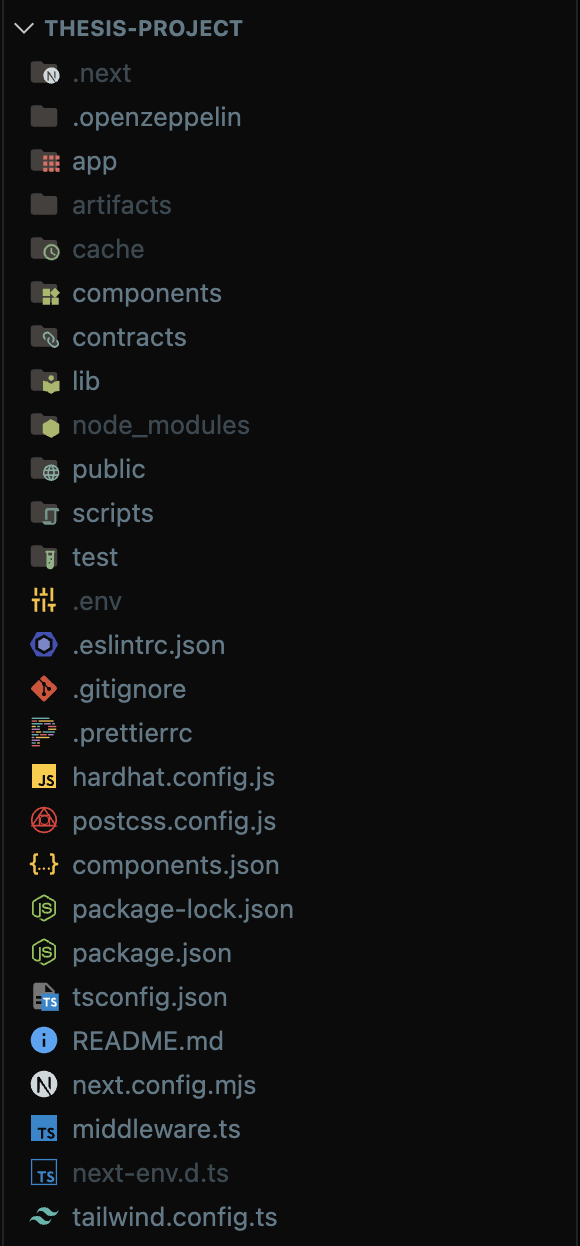
\includegraphics[scale=0.3]{src/images/folder-structure.png}
       \caption{Хөгжүүлэлтийн орчин}
   \end{minipage}
   \begin{minipage}[h!t]{0.5\textwidth}
      \raggedright
      \begin{itemize}
         \item \textbf{components} - React компонентууд
         \item \textbf{lib} - Хэрэглэгчийн талын шаардлагатай код туслах функцууд
         \item \textbf{app} - NextJS дээрх хуудаснууд
         \item \textbf{public} - Статик зураг, файлууд
         \item \textbf{scripts} - Ухаалаг гэрээний хөгжүүлэлтийн холбоотой  javascript файлууд
         \item \textbf{contracts} - Ухаалаг гэрээний файлууд
      \end{itemize}
  \end{minipage}
\end{figure}

\subsection{Ухаалаг гэрээн хөгжүүлэлт}
Миний төсөл нэг ухаалаг гэрээнээс бүтнэ. Ухаалаг гэрээг Solidity хэл дээр бичсэн бөгөөд Ethereum  блокчэйн дээр байршуулсан. Уг ухаалаг гэрээ нь цахим файлууд болон тэдгээртэй холбоотой лицензүүдийг төлөөлдөг Файл ба Лиценз гэсэн хоёр бүтцийг тодорхойлсон. Файл бүтэц  нь id, эзэмшигчийн хаяг, файлын нэр, дэлгэрэнгүй, ангилал, шифрлэсэн файлын хэш, файлын хэмжээ, үүсгэсэн хугацаа зэрэг атрибутуудыг агуулна. Лиценз бүтэц нь лицензийн дугаар, бүтээл эзэмшигчийн хаяг, лиценз эзэмшигчийн хаяг, файлын нэр, дэлгэрэнгүй, ангилал, шифрлэсэн файлын хэш, файлын хэмжээ, үүсгэсэн хугацааны  зэрэг атрибутуудыг агуулна.
Мөн дараах функцүүдтэй:

\begin{table}[h!]
	\centering
   \begin{tabularx}{\textwidth}{|p{0.4\textwidth}|X|}
		\hline
		 \textbf{createFile}& Цахим бүтээлийн мэдээллийг бичих
	\\ \hline \textbf{getAllPublicFiles} & Оруулсан бүх цахим бүтээлийн мэдээллийг авах
	\\ \hline \textbf{getAllUserFiles} &  Хэрэглэгчийн оруулсан цахим бүтээлийн мэдээллийг авах
	\\ \hline \textbf{getAllUserLicenses} & Хэрэглэгчийн эзэмшиж буй цахим бүтээлийн лицензүүдийг авах
	\\ \hline \textbf{getPublicFileById} & Цахим бүтээлийн мэдээллийг дугаараар нь авах
	\\ \hline \textbf{requestLicense} & Цахим бүтээлийг авах бүтээлийн эзэмшигч рүү лицензийн хүсэлт илгээх
	\\ \hline \textbf{approveLicenseRequest} & Өөрийн цахим бүтээлд ирсэн хүсэлтийг зөвшөөрөх
	\\ \hline \textbf{rejectLicenseRequest} & Өөрийн цахим бүтээлд ирсэн хүсэлтээс татгалзах
	\\ \hline \textbf{getFileOwnerLicenseRequests} & Бүтээлийн эзэмшигчид ирсэн хүсэлтүүдийг авах
	\\ \hline \textbf{isFileOwnedOrLicensed} & Цахим бүтээлийн эзэмшигч эсэх эсвэл түүний лицензийг авсан эсэхийг шалгах
	\\ \hline \textbf{generateUniqueLicense} & Лицензэд өвөрмөц дугаар бий болгох                                                             \\ \hline
	\end{tabularx}
\end{table}

\newpage
\subsection{Ухаалаг гэрээг блокчэйнд этереум байршуулах}
\lstinputlisting[language=TypeScript,caption=Ухаалаг гэрээг блокчэйнд байршуулах,basicstyle=\linespread{0.6}\ttfamily,frame=single]{src/code/deploy.js}

\subsection{Lit protocol-н файл шифрлэлт болон хандалтын хяналтын нөхцөл}
Lit Protocol-оор дамжуулан клиент талд файлыг шифрлэх ба блокчэйнд байршуулсан ухаалаг гэрээний функцийг ашиглан файлыг зөвхөн бүтээл эзэмшигч эсвэл тухайн бүтээлд хандах лиценз авсан хэрэглэгч эсэхийг батлагаажуулан файлын шифрлэлтийг тайлан харах боломжтойгоор хандалтын хяналтын нөхцөлийг тодорхойлсон.

\lstinputlisting[language=TypeScript,caption=Lit protocol-н файл шифрлэлт болон хандалтын хяналтын нөхцөл,basicstyle=\linespread{0.6}\ttfamily,frame=single]{src/code/lit.ts}


\subsection{Файлыг IPFS-д хадгалах}
\lstinputlisting[language=TypeScript,caption=Файлыг IPFS-д хадгалах,basicstyle=\linespread{0.6}\ttfamily,frame=single]{src/code/uploadIpfs.ts}

\subsection{Ухаалаг гэрээний өгөгдлийг унших}
Wagmi-н тодорхойлсон React Hook-г ашиглан цахим бүтээл эзэмшигчийн оруулсан бүтээлүүдийг ухаалаг гэрээнээс уншина.
\lstinputlisting[language=TypeScript,caption=Ухаалаг гэрээний өгөгдлийг унших,basicstyle=\linespread{0.6}\ttfamily,frame=single]{src/code/getUserFiles.ts}


\newpage
\section{Үр дүн}
Хөгжүүлэлтийг дээрх бүлэг сэдвүүд дээр тодорхойлсон шинжилгээ, зохиомжийн дагуу хийсэн болно. Системийн интерфейс дараах байдлаар харагдана.

\begin{figure}[h!]
	\centering
	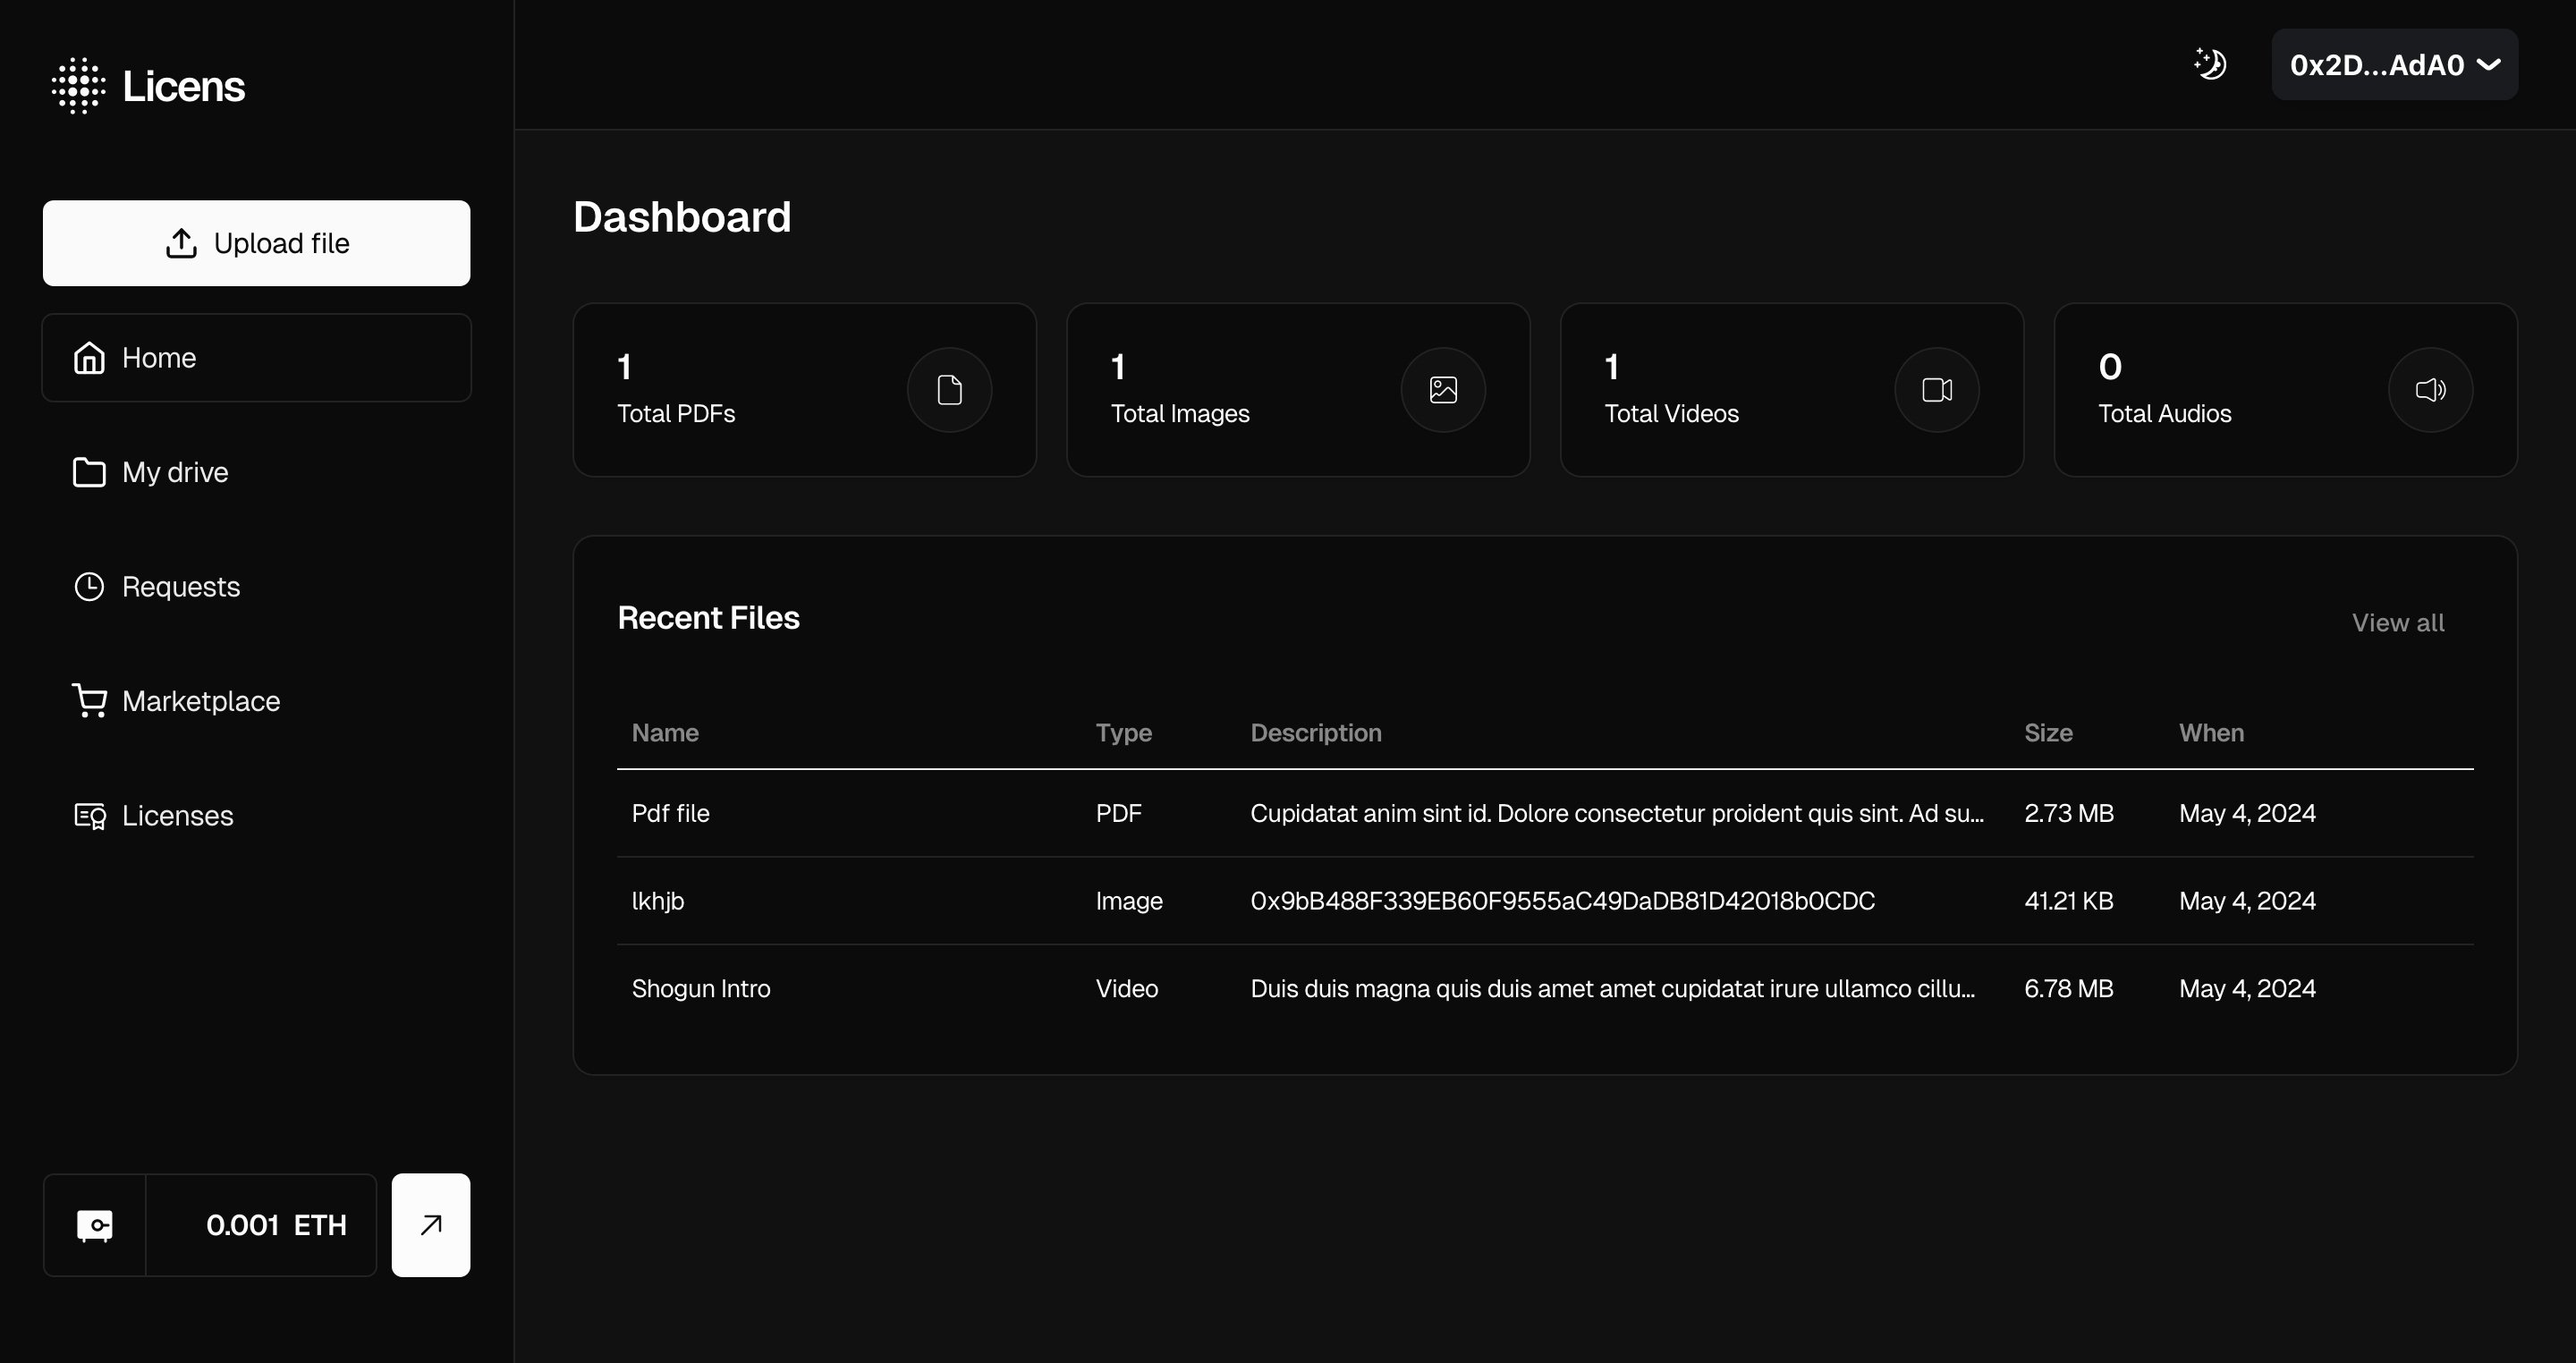
\includegraphics[scale=0.15]{src/images/dashboard.png}
	\caption{Хэрэглэгчийн үндсэн хуудас}
\end{figure}

% \subsubsection{Цахим бүтээл оруулах хуудас}
\begin{figure}[h!]
	\centering
	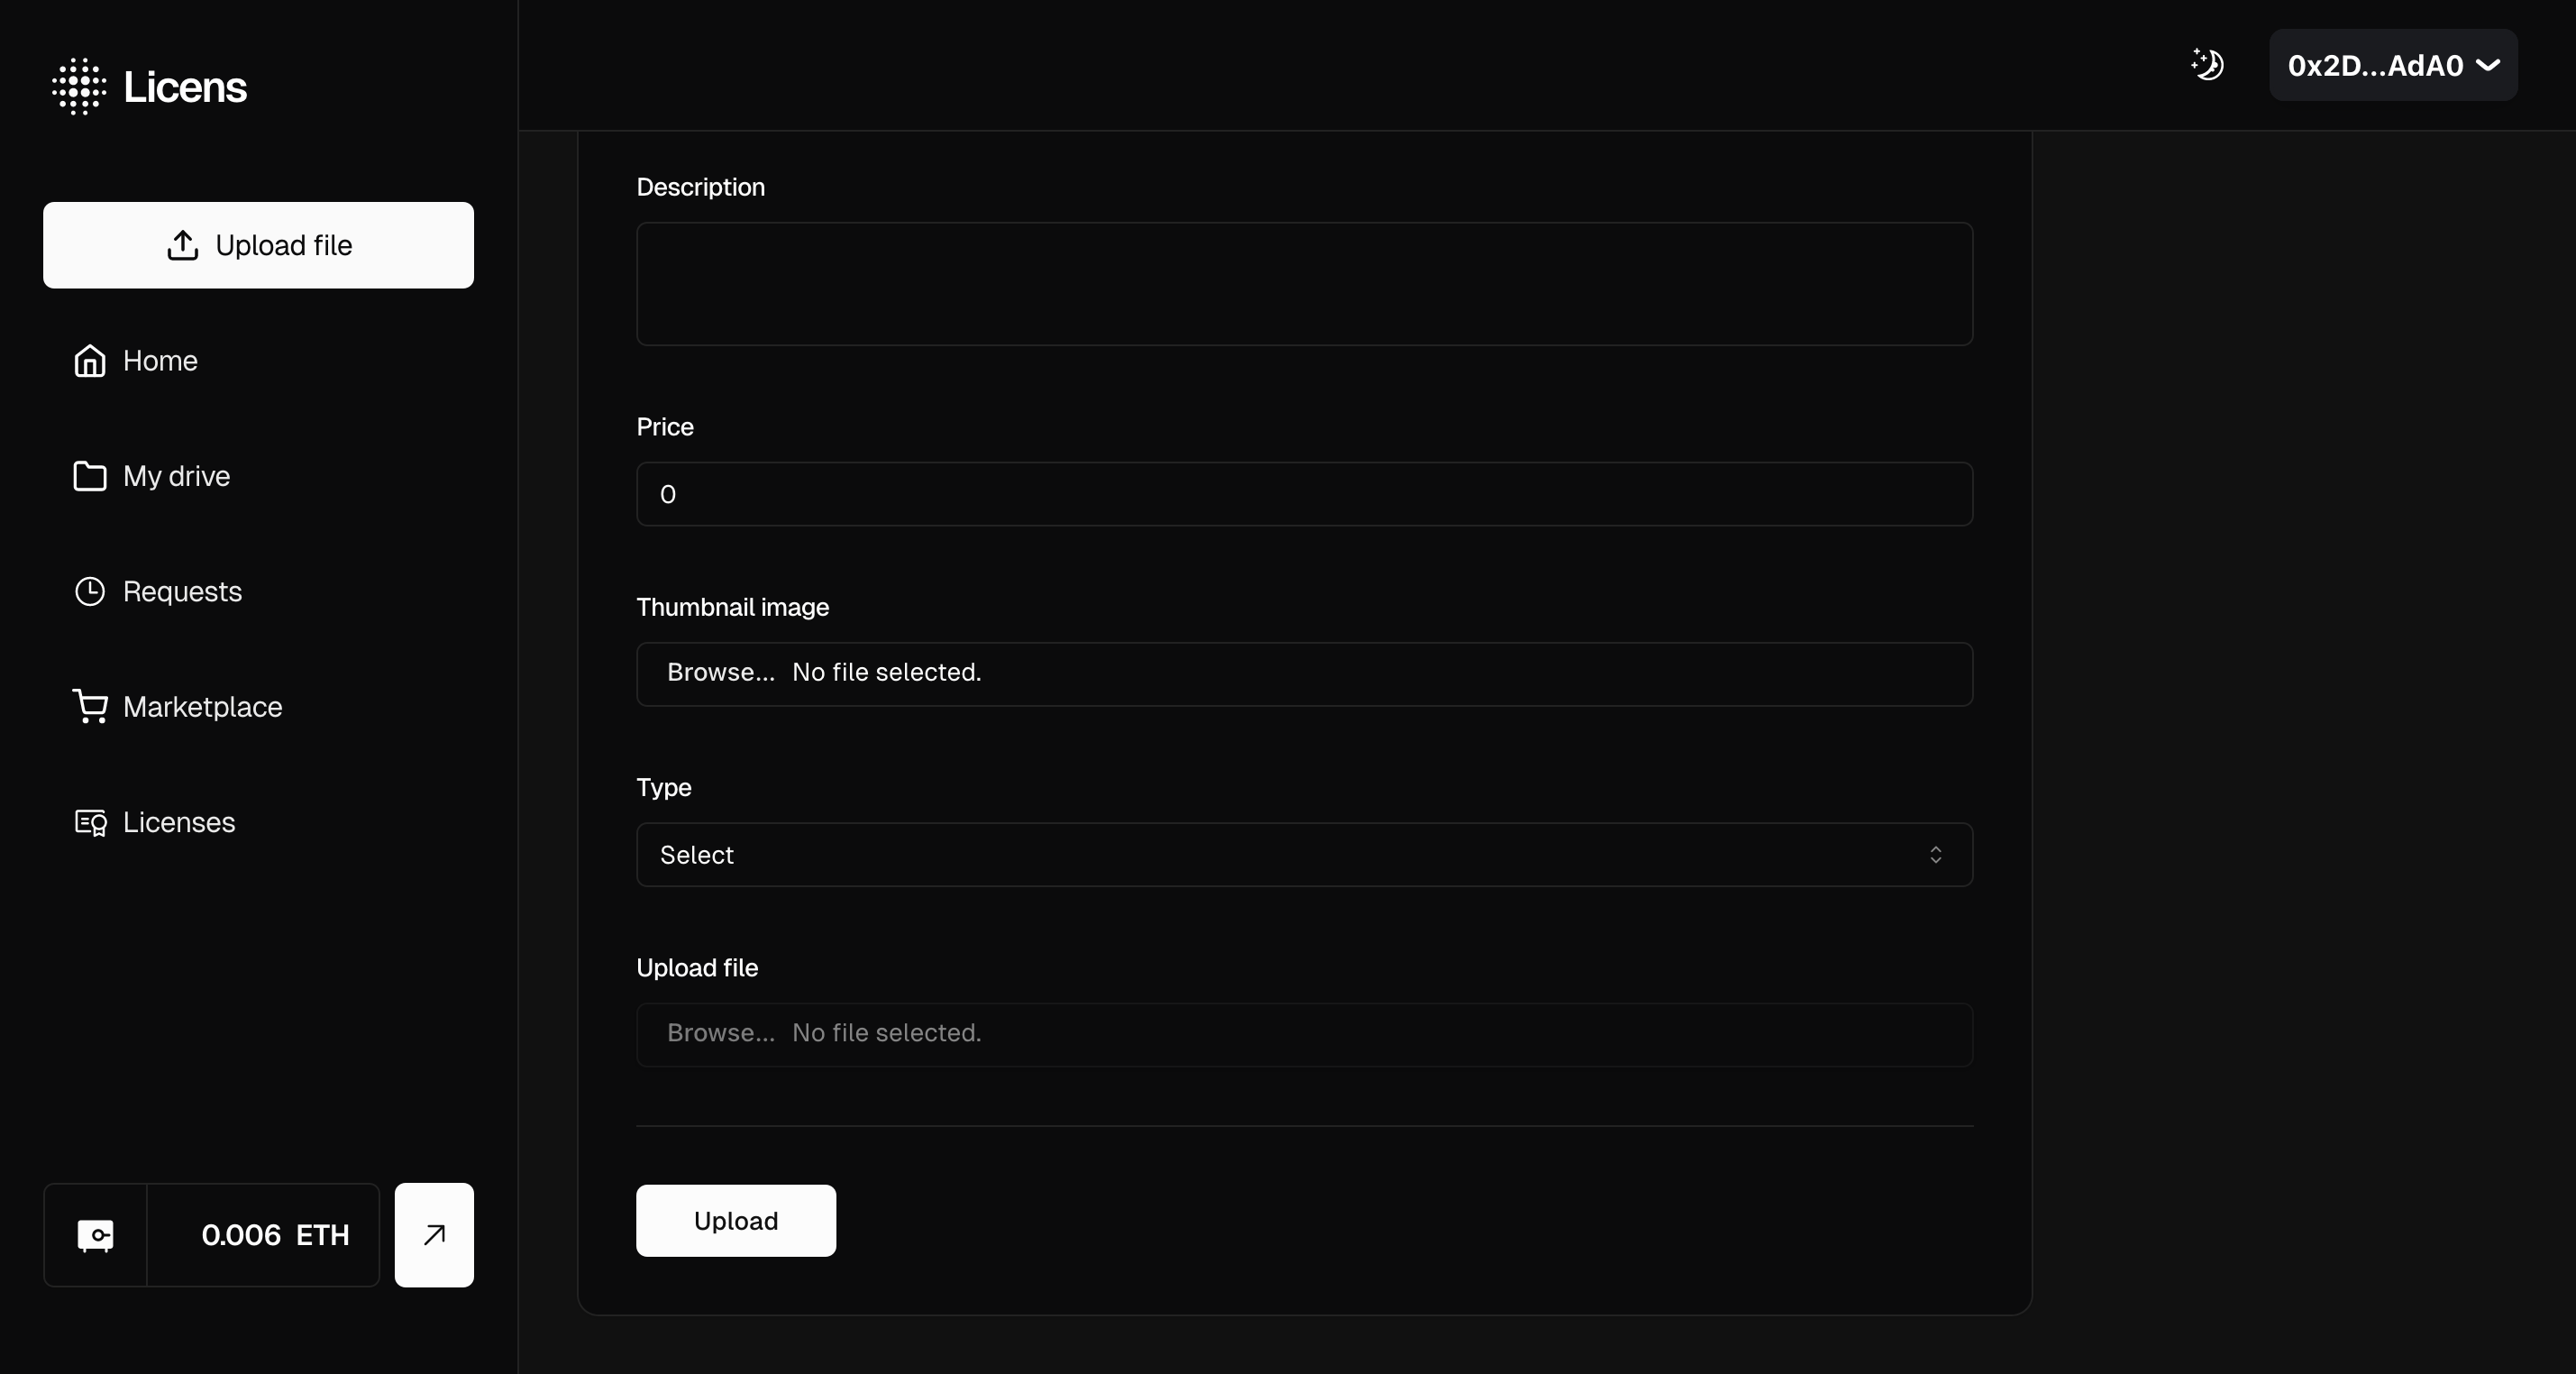
\includegraphics[scale=0.15]{src/images/upload.png}
	\caption{Цахим бүтээл оруулах хуудас}
\end{figure}

\begin{figure}[h!]
	\centering
	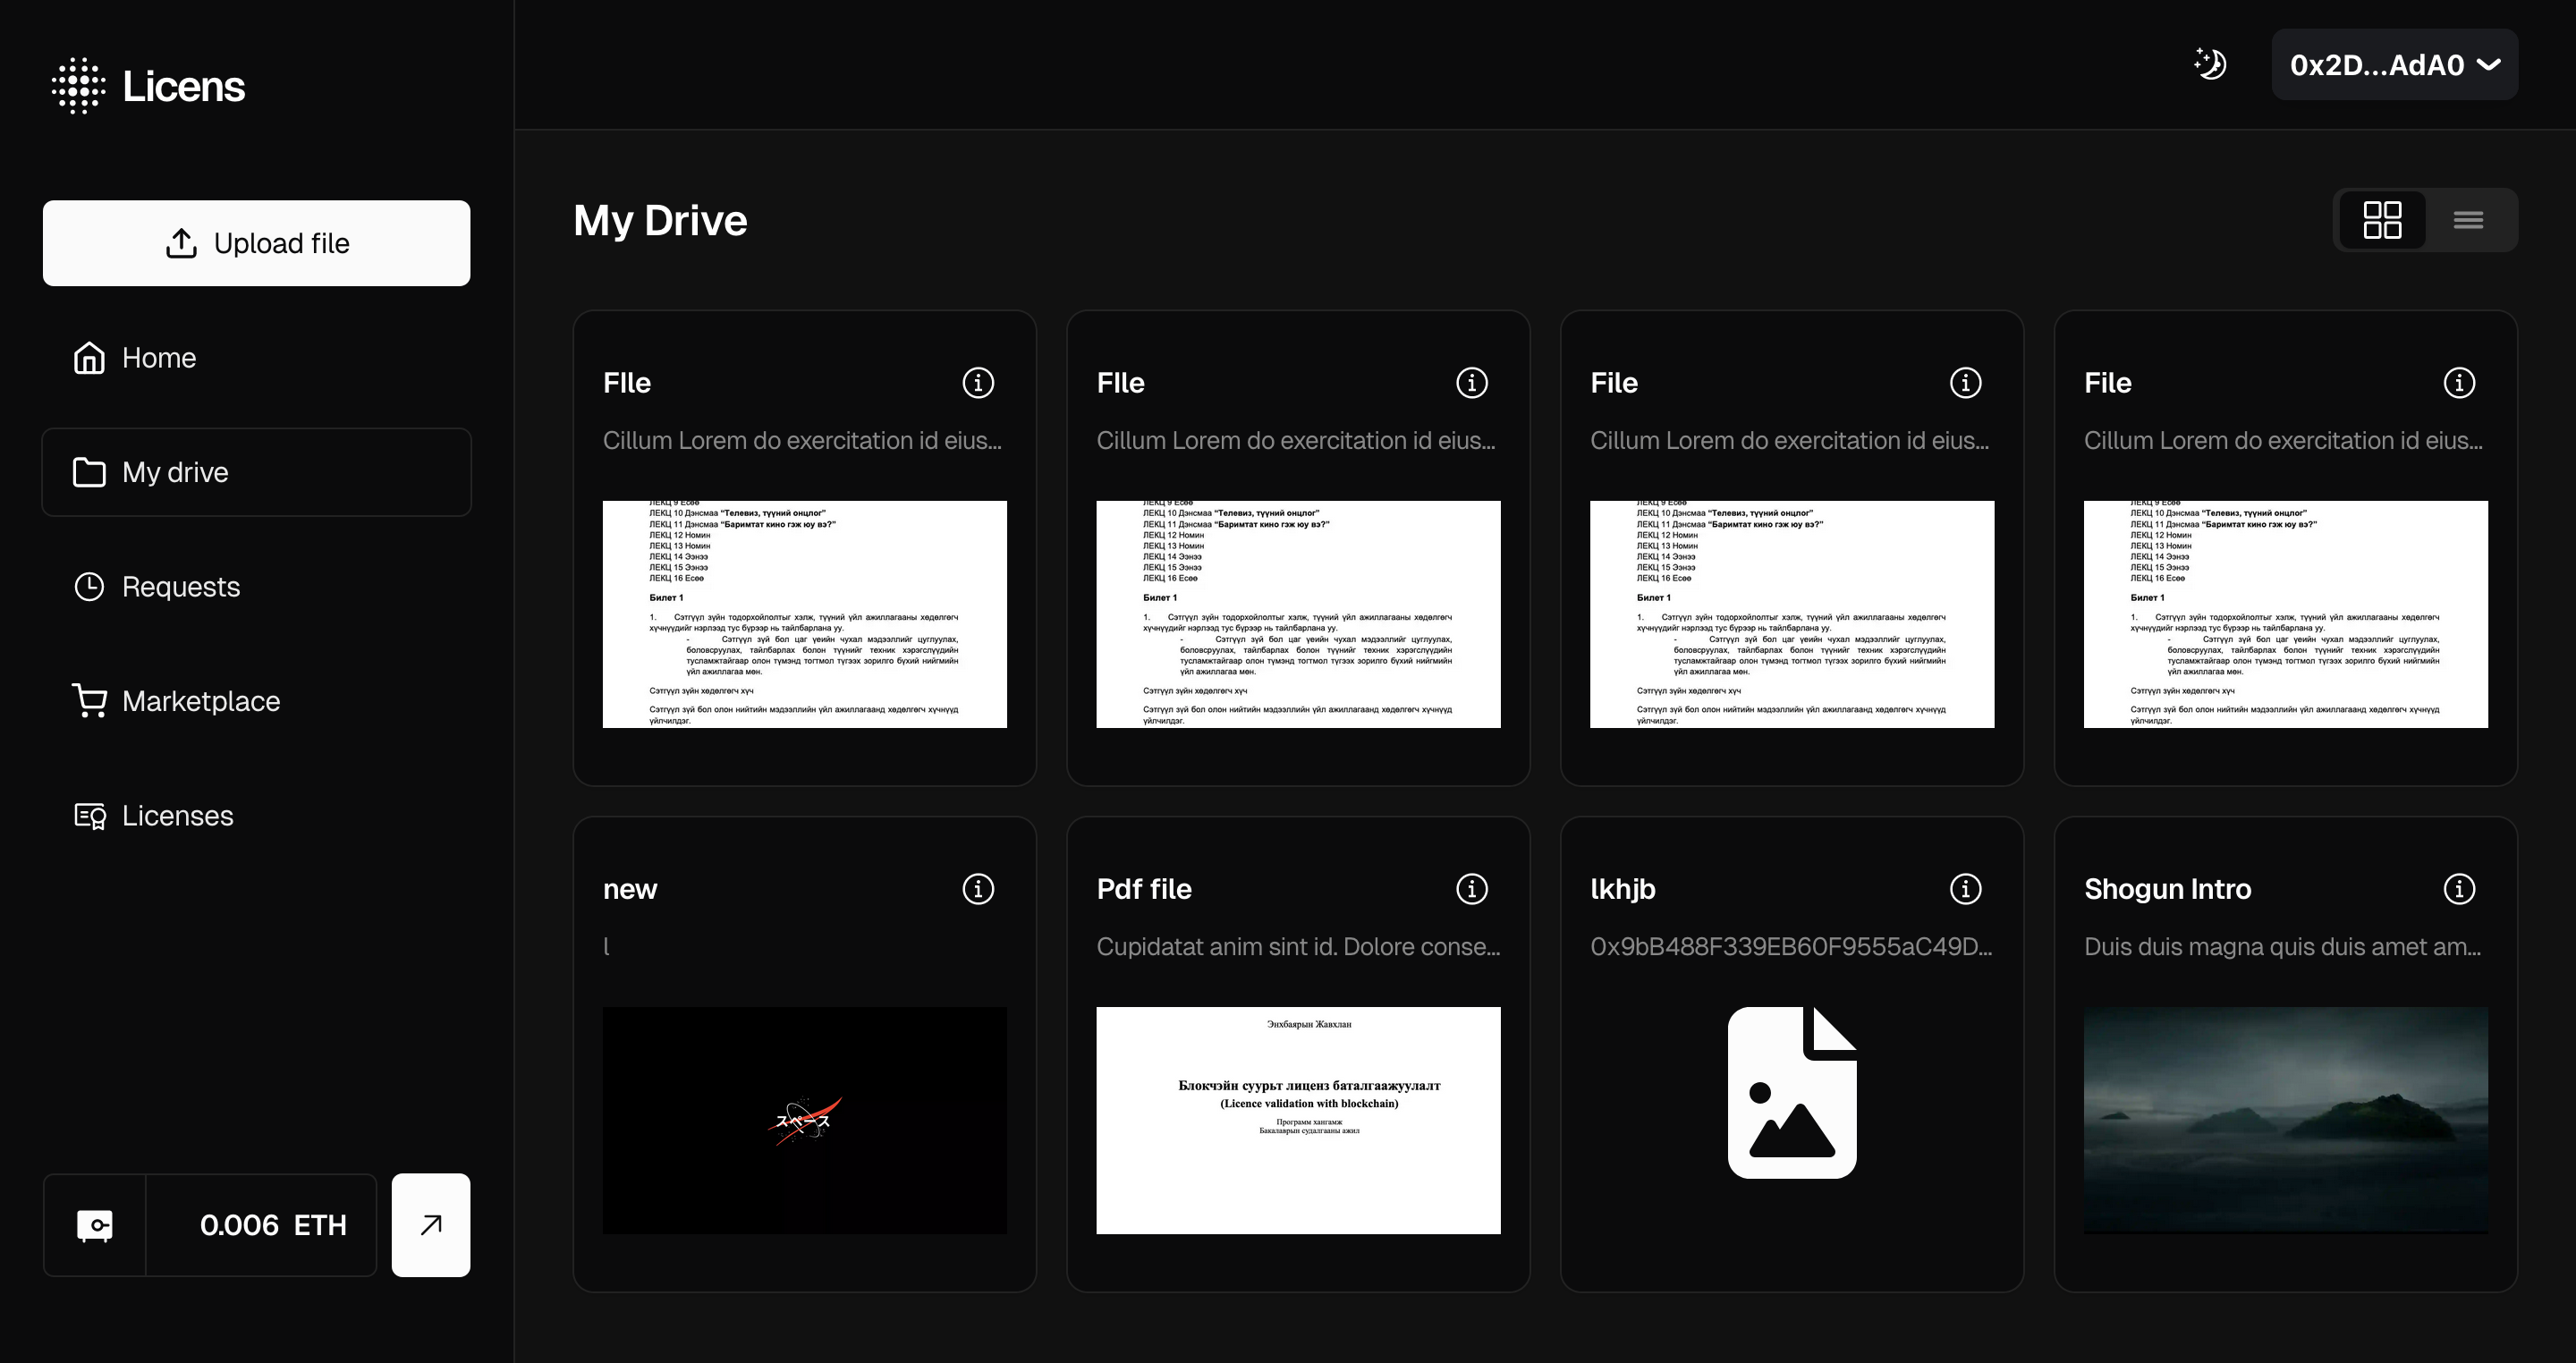
\includegraphics[scale=0.16]{src/images/drive.png}
	\caption{Миний сан хуудас}
\end{figure}

\begin{figure}[h!]
	\centering
	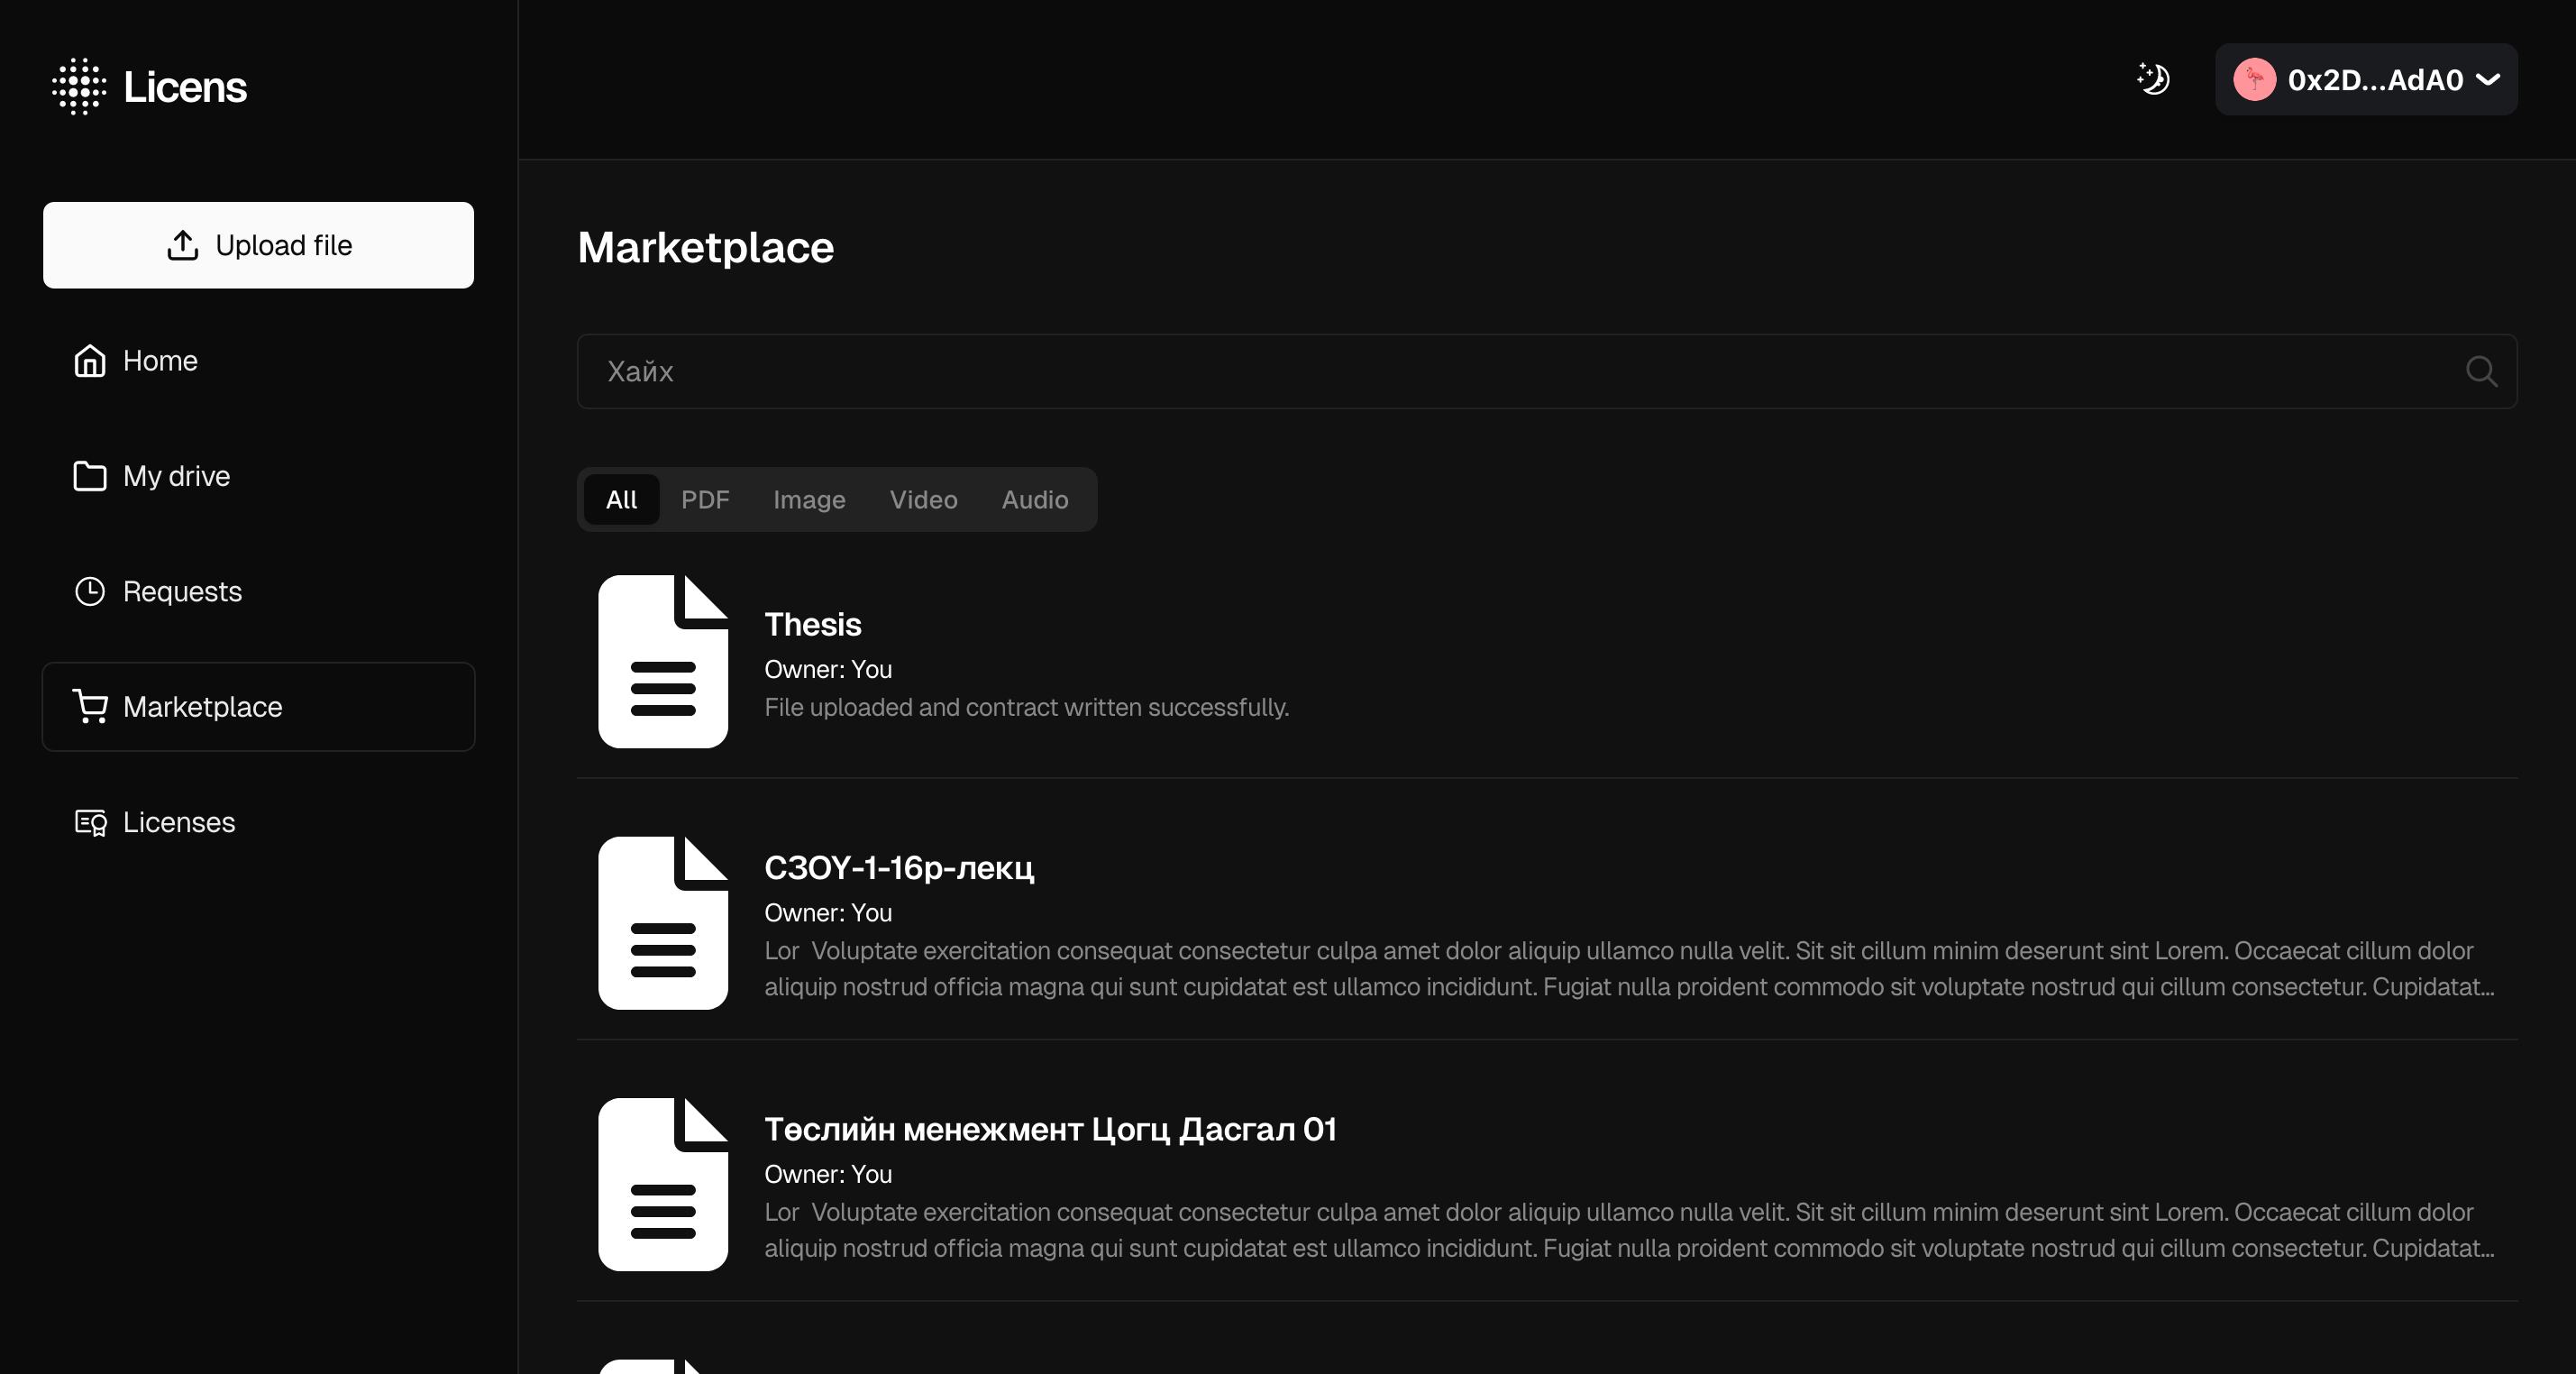
\includegraphics[scale=0.16]{src/images/marketplace.png}
	\caption{Marketplace хуудас}
\end{figure}

\begin{figure}[h!]
	\centering
	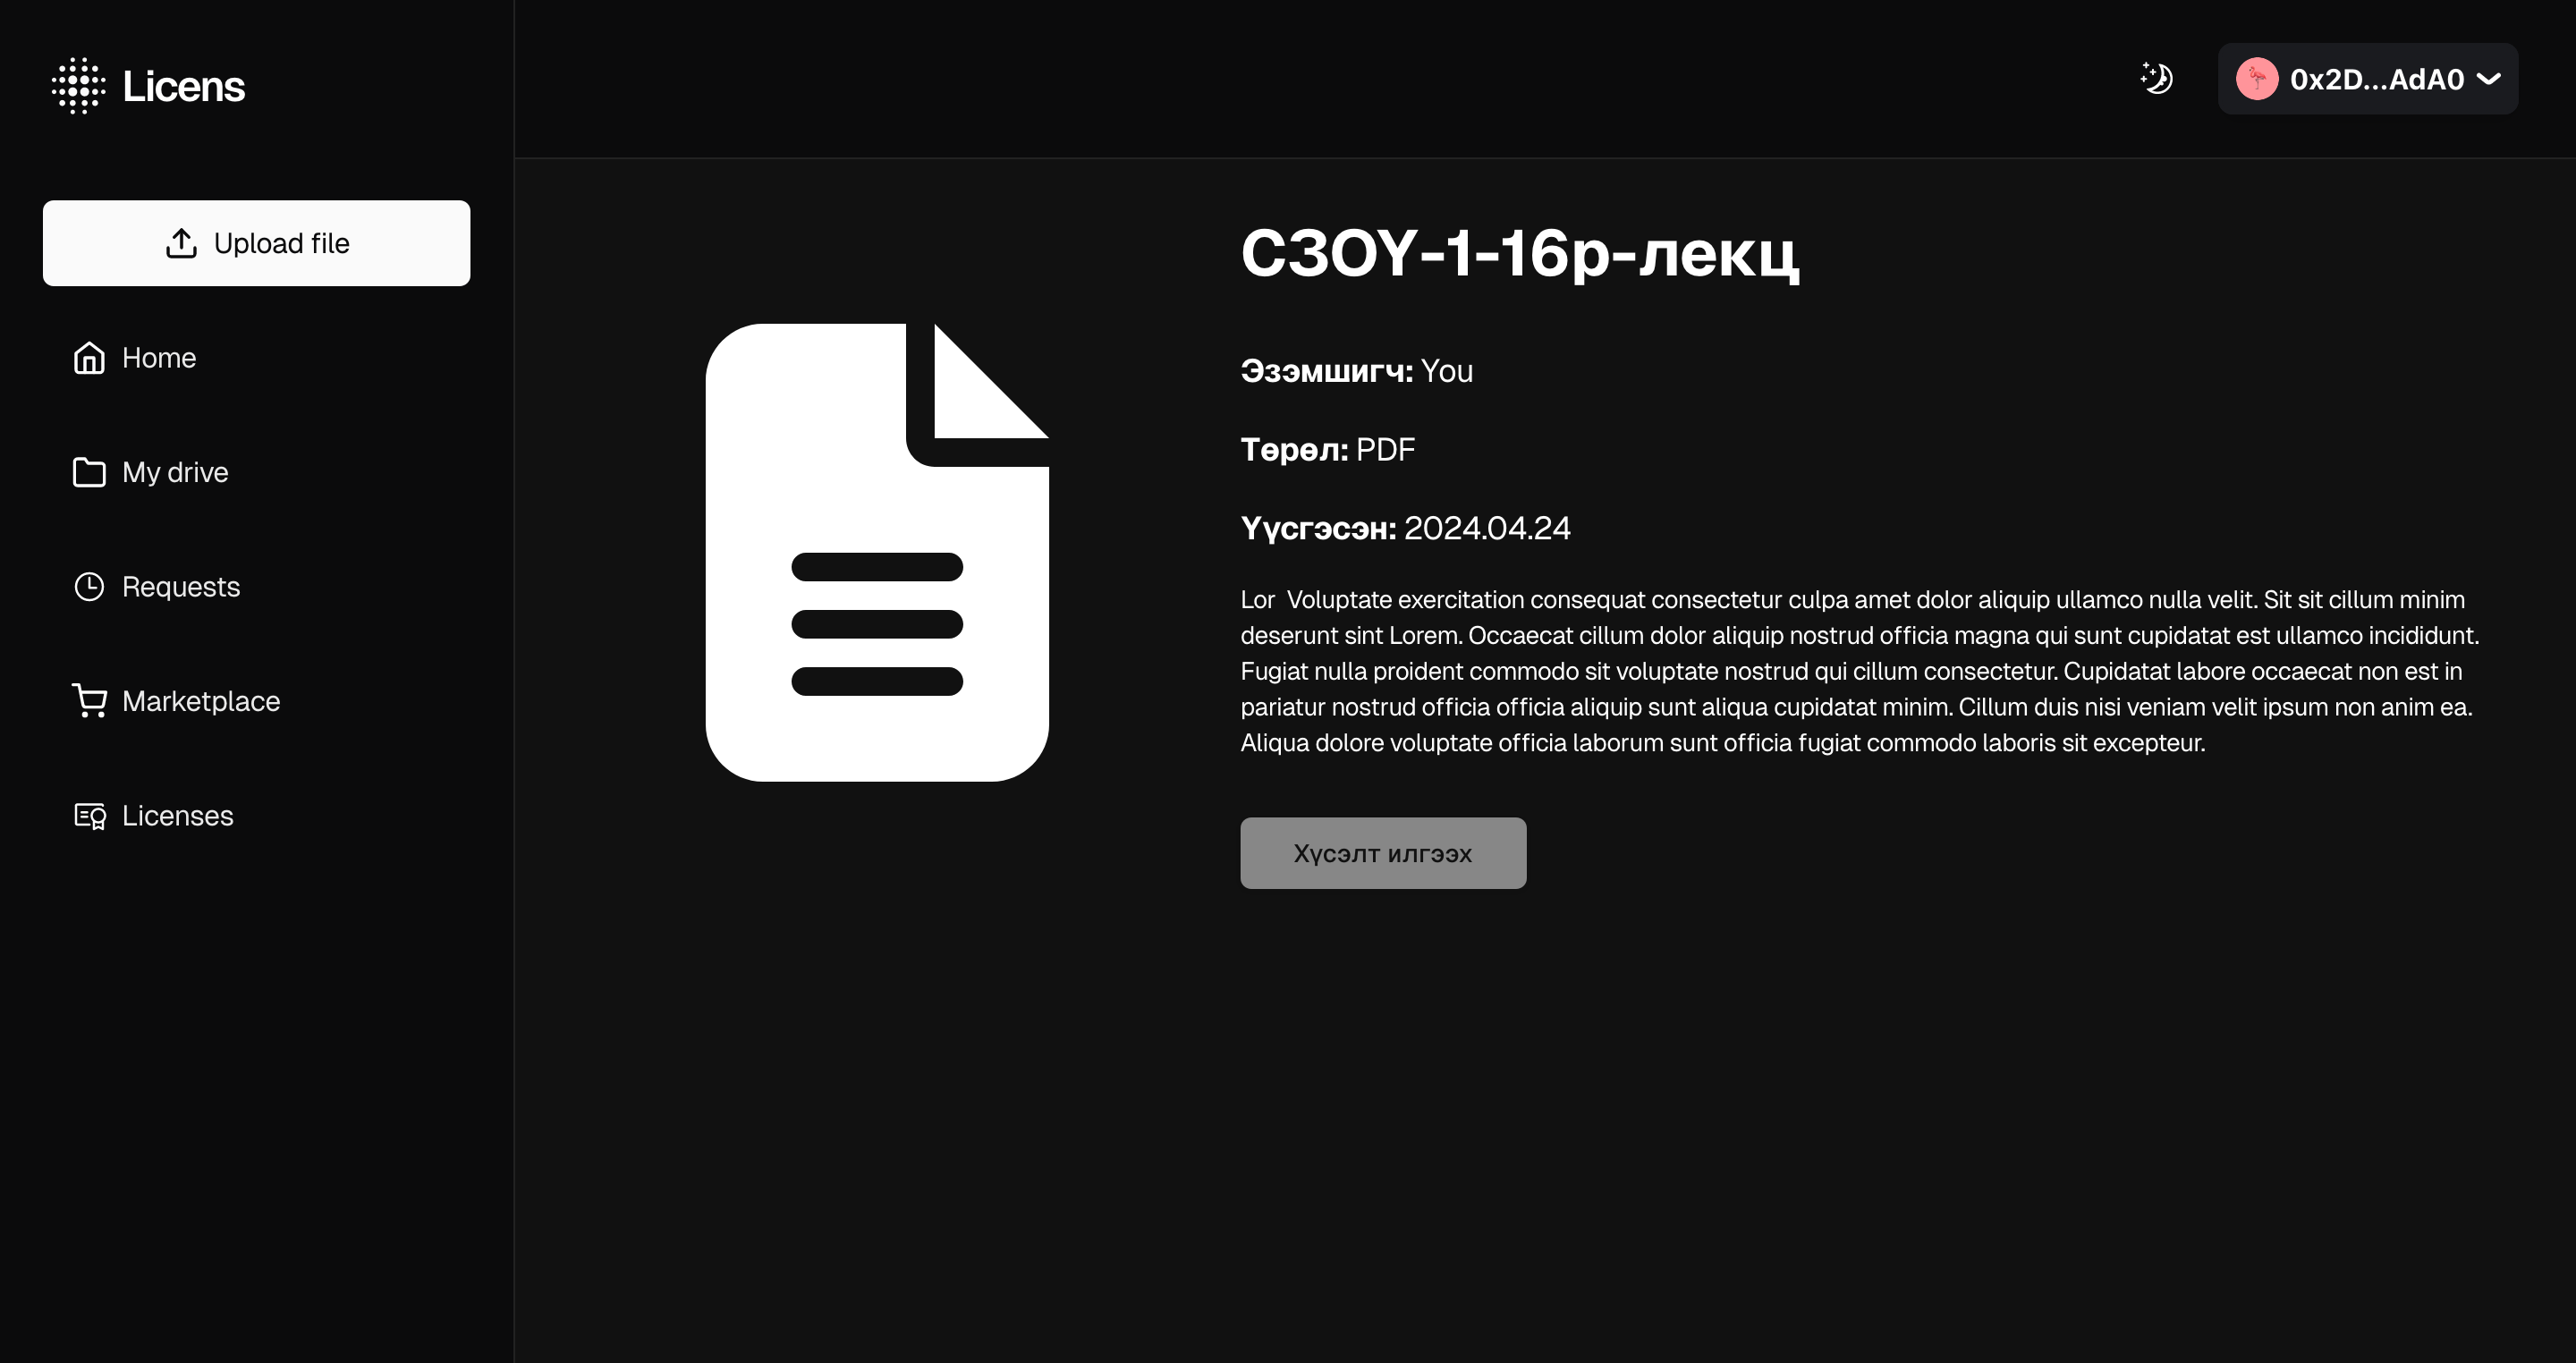
\includegraphics[scale=0.16]{src/images/marketplace-file.png}
	\caption{Marketplace дэх бүтээлийн хуудас}
\end{figure}

\begin{figure}[h!]
	\centering
	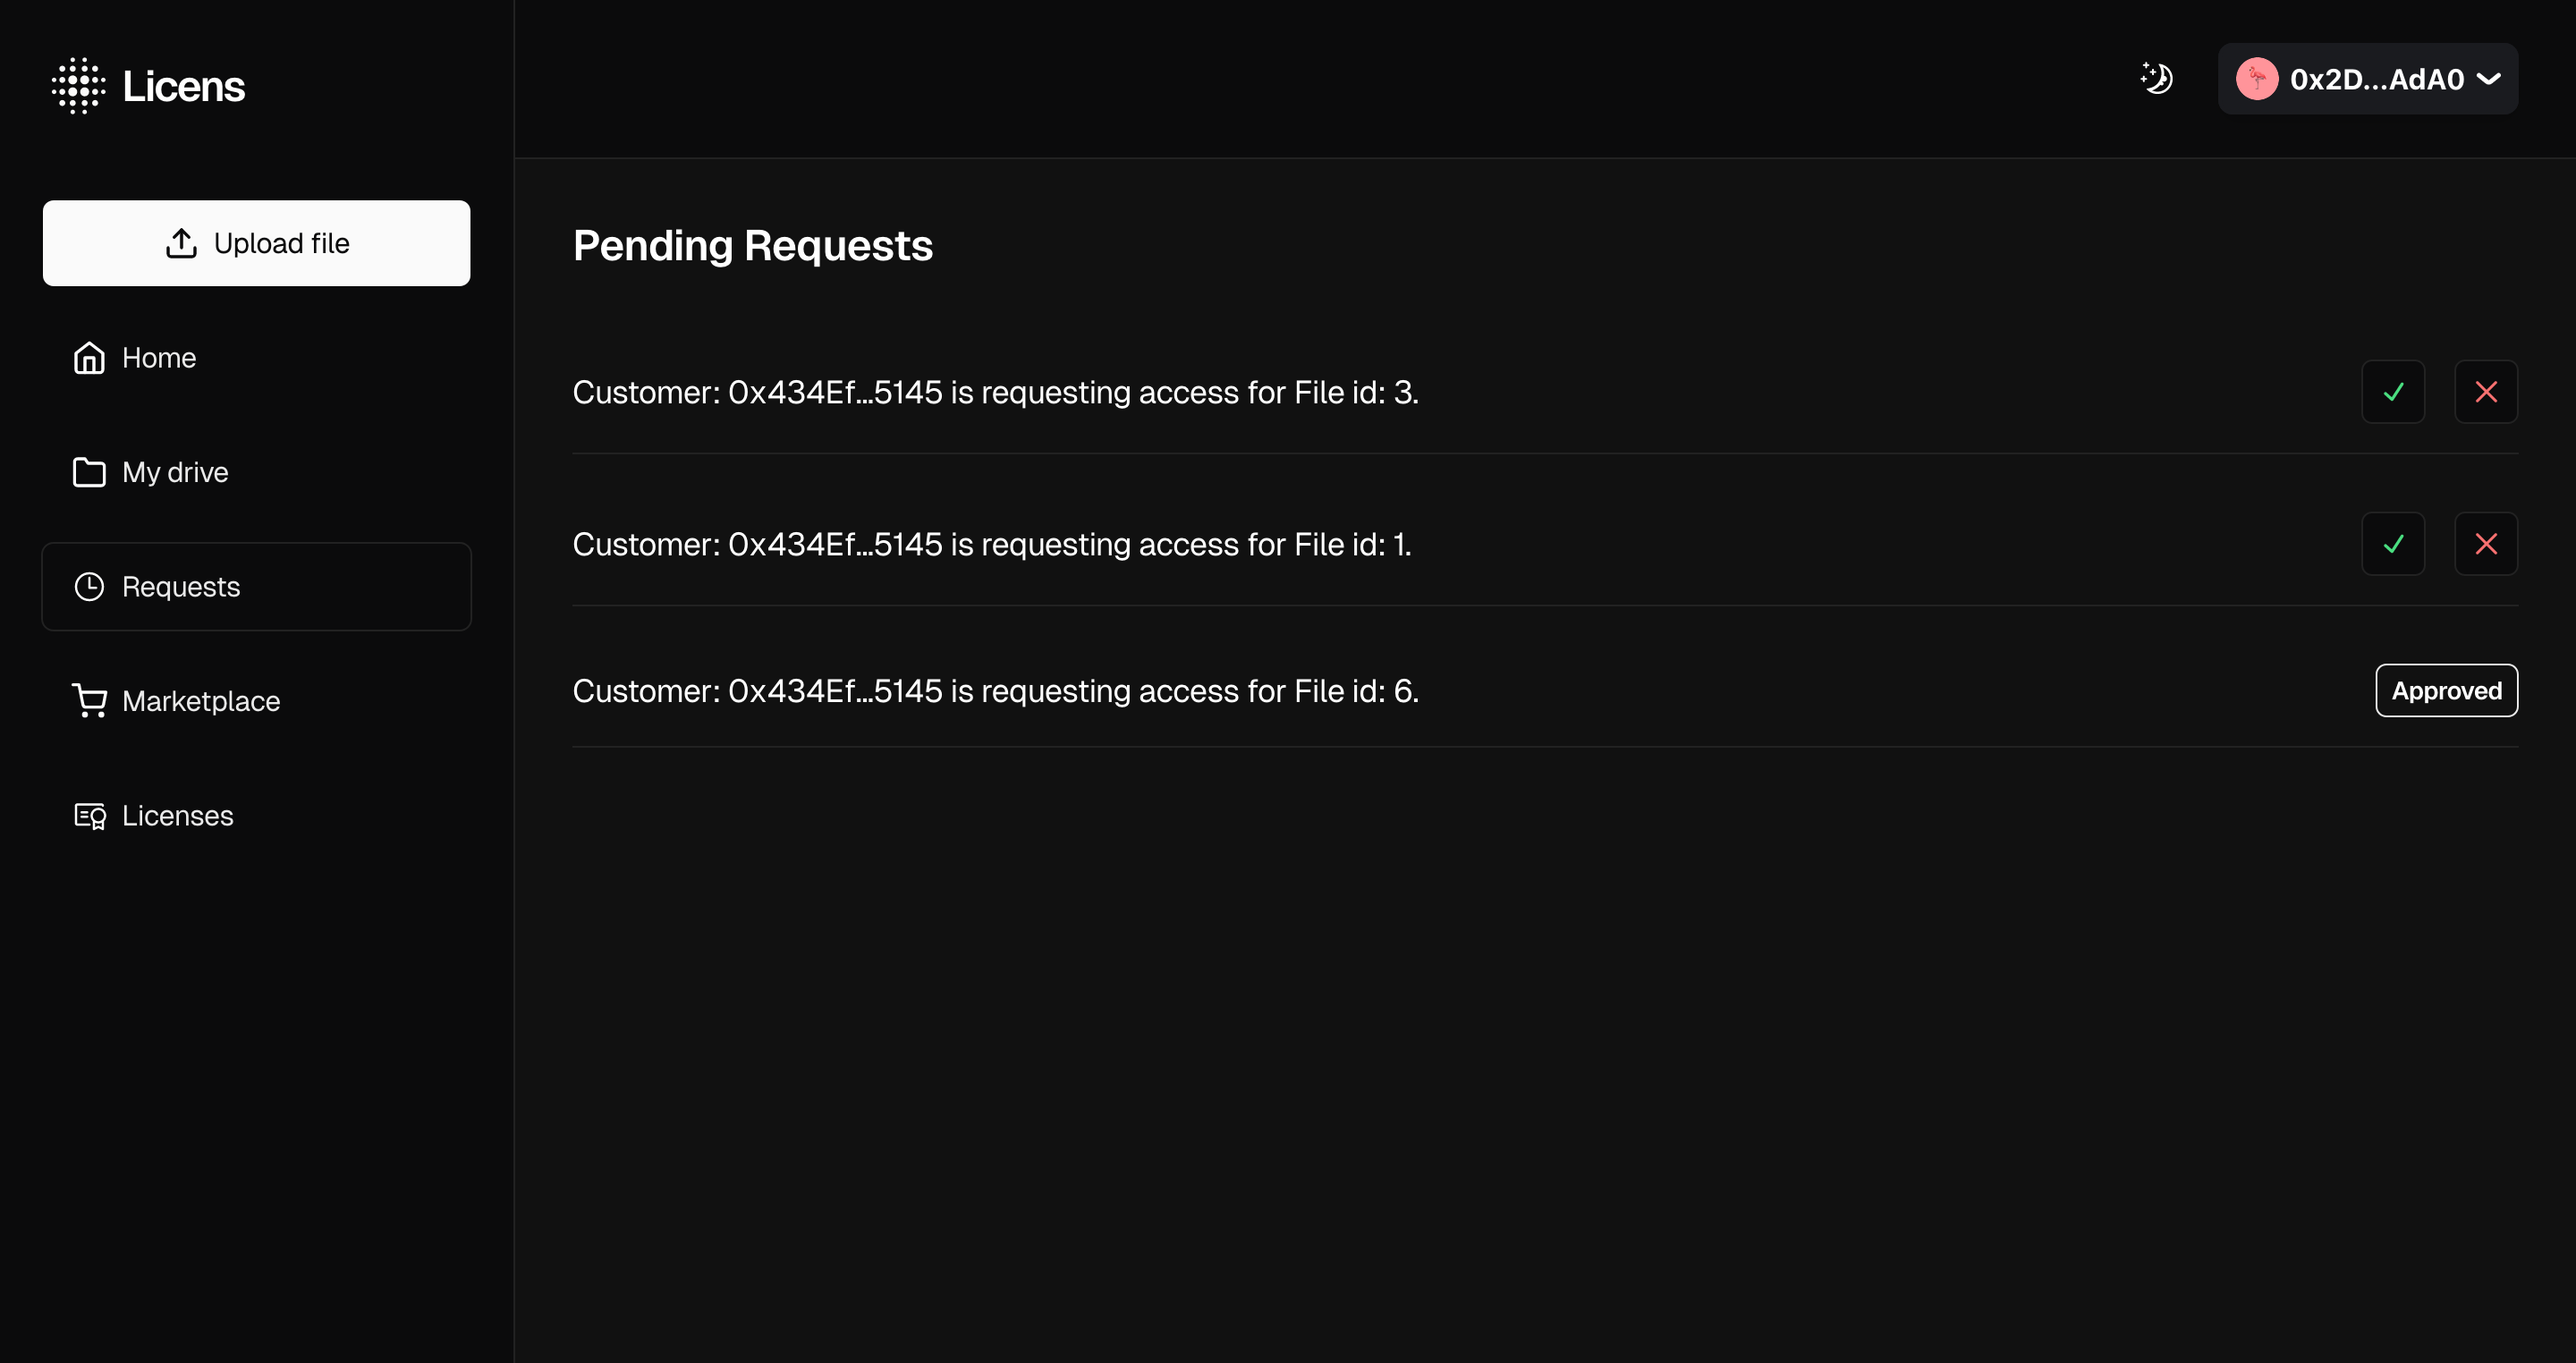
\includegraphics[scale=0.16]{src/images/requests.png}
	\caption{Лиценз хүсэлтийн  хуудас}
\end{figure}